\documentclass{amsart}

\usepackage{xeCJK}
\usepackage{amssymb}
\usepackage{graphicx}
\usepackage{amsmath}
\newtheorem{theorem}{Theorem}[section]
\newtheorem{lemma}[theorem]{Lemma}

\theoremstyle{definition}
\newtheorem{definition}[theorem]{Definition}
\newtheorem{example}[theorem]{Example}
\newtheorem{xca}[theorem]{Exercise}

\newcommand{\etal}{\textit{et al}.}
\newcommand{\ie}{\textit{i}.\textit{e}.}
\newcommand{\eg}{\textit{e}.\textit{g}.}
\newcommand{\sol}{\emph{Sol.}}
\newcommand{\q}{$}
\newcommand{\e}{\par From this we get:}


\theoremstyle{remark}
\newtheorem{remark}[theorem]{Remark}

\numberwithin{equation}{section}
%-------------------------------------------------------------
%-------------------------------------------------------------
%-------------------------------------------------------------
\begin{document}

\title[AMS Article Template]{ICARUS:A new type of NFT with infinite series convergence}
\author{Wang Chuwen}
%\address{59 Zhongguancun Street, Haidian District, Beijing, people's Republic of China}
%\curraddr{RENMIN University}
%\email{2018202114@ruc.edu.cn}
\thanks{Copyright © 2021- by wangchuwen,www.wangchuwen.com. All rights reserved}

%\subjclass[2010]{Primary}

\keywords{NFT,digital currency,crypto}

\date{2021-05-15}
\dedicatory{wenchuwangchuwen@gmail.com}
\begin{abstract}
    Icarus is an end-to-end encrypted digital currency. The emergence of ethereum smart contracts has allowed digital currencies to reach the 2.0 era. Existing currencies can be divided into two types according to the number of issues: total limited and total unlimited. In terms of anti-inflationary effect, the aggregate limited type of currency is more advantageous and therefore it is also believed that these cryptocurrencies are advantageous in the long run. Converting funds into a faster issuing currency, on the other hand, is considered a speculation, or a game of boondoggle.
\end{abstract}

\maketitle

\section{introduction}
\paragraph{
}
\begin{figure}[ht]
    \centering
    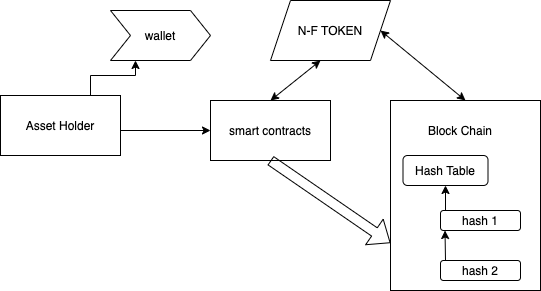
\includegraphics[scale=0.5]{icarusbc.png}
    \caption{Icarus Blockchain Concept}
    \label{fig:label}
\end{figure}



\end{document}